\cleardoublepage
\appendix
\chapter{Giao diện và hướng dẫn sử dụng công cụ}
Để bắt đầu sử dụng công cụ, ta gõ lệnh \texttt{python3 -W ignore server.py} từ thư mục gốc chứa mã nguồn của công cụ. Ở bước bắt đầu, giao diện công cụ hiển thị biểu ngữ bao gồm tên công cụ, tên tác giả, một cửa sổ trình duyệt Firefox, đồng thời cho phép người dùng chọn lỗ hổng bảo mật để kiểm thử như Hình  dưới đây.

Trong trường hợp lần đầu sử dụng công cụ, ta cần cài đặt phần mở rộng \texttt{y4t0g4m1.jar} trong đường dẫn \texttt{src/burp-extension}, chi tiết việc cài đặt thêm phần mở rộng Java có thể tham khảo tại \parencite{burp-suite-extension-setup}. Giao diện chính của phần mở rộng trên Burp Suite được mô tả như Hình \ref{fig:main-burp-extension-interface} dưới đây, chỉ đơn giản gồm một textbox để thiết lập địa chỉ máy chủ công cụ nhận request mẫu. Mặc định giá trị của trường này là \texttt{http://127.0.0.1:13337}, là địa chỉ máy chủ công cụ khi chạy trên localhost, khi ta triển khai công cụ lên một dịch vụ vps nào đó thì địa chỉ IP sẽ thay đổi, giá trị port \texttt{13337} vẫn phải được giữ nguyên. 
\begin{figure}[H]
  \centering
    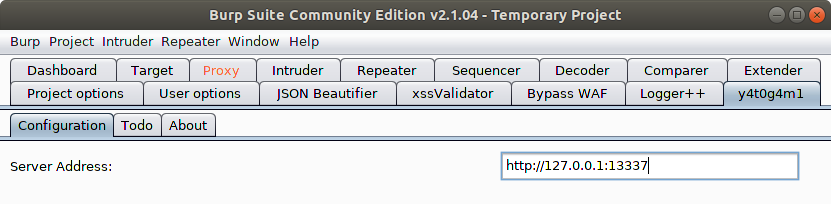
\includegraphics[width=\textwidth,keepaspectratio=true]{images/main-burp-extension-interface.png}
  \caption{Giao diện chính của phần mở rộng trên Burp Suite}
  \label{fig:main-burp-extension-interface}
\end{figure}
Sau khi khởi chạy công cụ webfuzzer và cài đặt phần mở rộng trên Burp Suite, ta tiến hành thiết lập proxy trên Burp Suite và trình duyệt web để bắt request mẫu như hướng dẫn tại \parencite{burp-suite-proxy}. Sau đó ta chuyển request mong muốn đến tab \texttt{Intruder} để tạo và gửi request mẫu đến máy chủ webfuzzer. Hình \ref{fig:send-base-request-1} mô tả quá trình này bằng cách thêm hoặc bỏ các kí tự ``\texttt{\$}'' bao quanh giá trị của tham số và chọn ``\texttt{Send to y4t0g4m1 webfuzzer}''.

Sau khi đã chọn loại lỗ hổng và gửi request mẫu đển webfuzzer, giao diện công cụ lần lượt hiển thị thông báo loại lỗ hổng sắp được kiểm thử (trong trường hợp này là \texttt{Time-based \acrshort{sqli}}) kèm theo các thiết lập của công cụ để phát hiện lỗ hổng đó, bao gồm tập tin chứa danh sách payload, đường dẫn chứa kết quả kiểm thử, các chuỗi dùng để so trùng trong response trả về, thời gian tối đa xử lí request. Sau đó là các kết quả kiểm thử đối với mỗi payload cụ thể và thông báo đã kiểm thử xong loại lỗ hổng này. Giao diện trong quá trình của kiểm thử của công cụ được thể hiện trong Hình 
Hình cũng thể hiện một số kết quả kiểm thử mà công cụ phát hiện thấy. Mỗi kết quả được in ra bao gồm các thành phần như sau.
\begin{itemize}
    \item \textbf{Kết quả kiểm thử} được đặt trong cặp ngoặc vuông, có thể là \texttt{[passed]} trong trường hợp payload khai thác thành công lỗ hổng, \texttt{[failed]} trong trường hợp payload không khai thác thành công hoặc \texttt{[skeptical]} trong trường hợp payload gây ra lỗi hoặc ngoại lệ khả nghi trong quá trình gửi request, chưa xác định được là có khai thác lỗ hổng thành công hay không, cần được hậu kiểm lại bằng tay.
    \item \textbf{Mã trạng thái HTTP} của response trả về, thường là \texttt{200} trong trường hợp request được gửi thành công hoặc các mã lỗi \texttt{401}, \texttt{404}, \texttt{500},... khi có sự cố trong quá trình xử lí request ở ứng dụng web mục tiêu.
    \item \textbf{Độ dài nội dung (content length)} của response trả về, \textbf{thời gian xử lí} của request tính theo giây và payload tương ứng được gửi theo request. Lỗi hoặc ngoại lệ trong quá trình xử lý request (nếu có) cũng được xuất ra ngay sau dòng kết quả kiểm thử.
\end{itemize}
Những kết quả kiểm thử được đánh dấu là \texttt{[passed]} hoặc \texttt{[skeptical]} sẽ được ghi lại trong nhật kí hoạt động kèm theo ngày giờ và loại lỗ hổng kiểm thử thành từng tập tin văn bản lưu trong thư mục \texttt{logs} trong đường dẫn gốc. Các tập tin nhật kí này chứa \acrshort{poc} khai thác lỗ hổng bao gồm request mẫu và các payload đã \texttt{[passed]} hoặc \texttt{[skeptical]} như Hình 
% TODO: Viết thêm hướng dẫn modify burp extension trong đây và trong README.md